\section{Introduction}
\label{sec:intro}

As computing platforms migrate to clusters of increasingly larger scale of microprocessors,
 applications need to manage the distributed memories of the processors via explicit
message-passing runtimes, for example, MPI, to attain high performance.
The relative latency and bandwidth of the communication network in relation to the compute capacity of processors
are often hard to predict a priori and may change dramatically from one system to the next.
Even on supercomputers comprising homogeneous nodes,
system noise is increasing on each node because of aspects such as power management, deeper memory hierarchies, and sharing of hardware such as caches and network. The ``equal work means equal time" paradigm is no longer relevant on most systems, and load imbalance increasingly becomes the common scenario even on applications that are symmetrically structured.
Consequently, bulk-synchronous communication, where all processes synchronize frequently, is no longer a valid option for high-performance MPI applications.
Application performance is often critically determined by its ability to flexibly overlap communications with local computations,
thereby minimizing wait time.


This paper aims to automatically enable the use of nonblocking latency-hiding techniques to overlap local computation with remote communication in MPI applications, thereby enhancing their overall efficiency and performance portability.
%through a framework that systematically combines analytical performance modeling of the application execution flow and compiler-assisted safety and profitability analysis.
To illustrate the optimization, Figure~\ref{fig:ft_loop} shows the
structure of the NAS FT benchmark~\cite{npb}, which applies fast
Fourier transform (FFT) to a 3D matrix through a loop that interleaves
the computation of scaling the input matrix with a collective
communication of MPI\_Alltoall to exchange data among the
processes. This is then followed by a final transposition of the
resulting matrix.  The clear separation of computation and
communication phases makes the algorithm design easy to implement and
maintain.  Additionally, the communication buffers can be reused
across different loop iterations, saving memory.  However, the
blocking MPI communication requires that all processes wait while the
MPI\_Alltoall operation is in progress.  Consequently, unless the
application is executed on a platform with the fastest network
connections, its performance is likely to suffer because of the
excessive wait time.

\begin{figure}
  \centering
  \begin{subfigure}[b]{0.25\textwidth}
    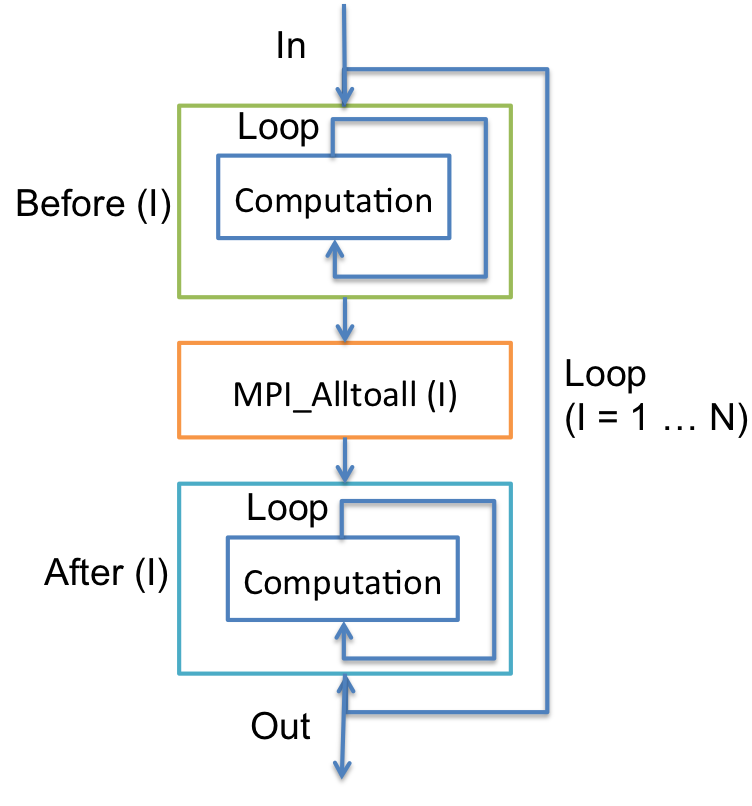
\includegraphics[width=1\textwidth]{fig/ft_loop.png}
    \caption{Before optimization}
    \label{fig:ft_loop}
  \end{subfigure}%
  \begin{subfigure}[b]{0.232\textwidth}
    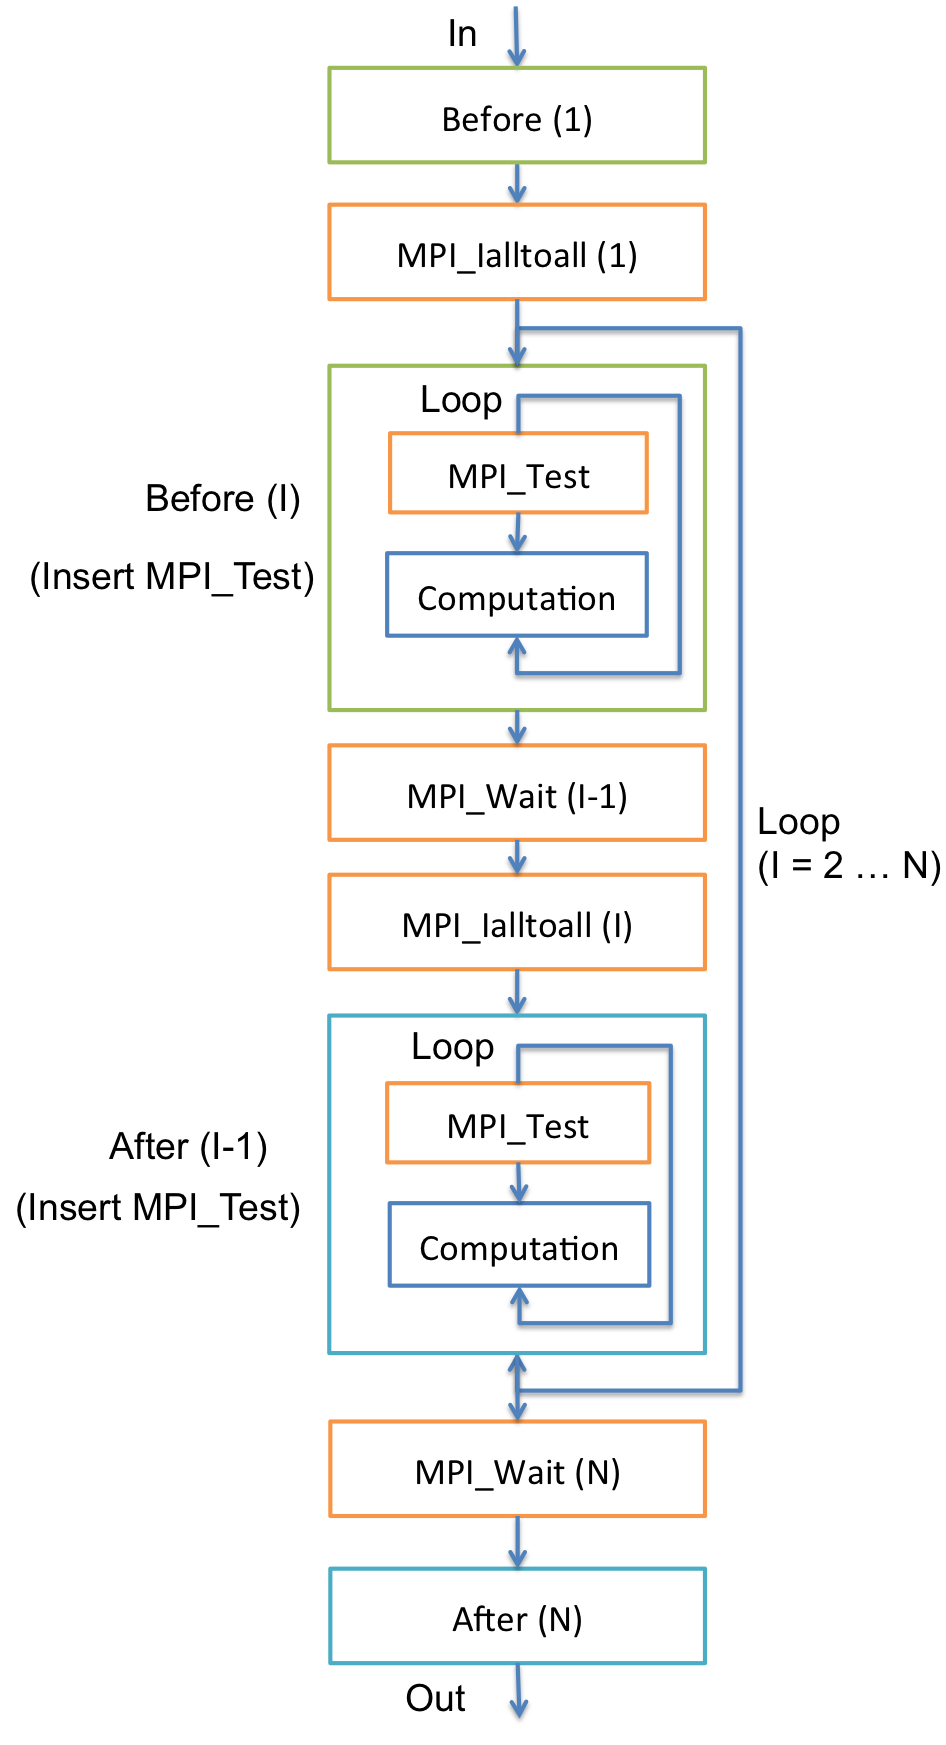
\includegraphics[width=1\textwidth]{fig/ft_cco.png}
    \caption{After optimization}
    \label{fig:ft_cco}
  \end{subfigure}
  \caption{Optimizing NAS FT by
    overlapping computation with communication (Before(i)/After(i) are computations before/after the MPI communication of the $i$th loop iteration)}
\label{fig:ft}
\end{figure}

Figure~\ref{fig:ft_cco} illustrates how the structure
in~\ref{fig:ft_loop} may be modified to better overlap computation
with communication.  In particular, the MPI\_Alltoall operation is
decoupled into two finer-grained operations: a nonblocking
MPI\_Ialltoall and a blocking MPI\_Wait.  Then, the loop is modified
so that Before(i), which multiplies a local matrix with a
time-evolution array and then saves a transpose of the matrix into a
local buffer to be communicated to other processors, and
MPI\_Ialltoall(i), which exchanges the local transposes among different
processes, are essentially moved so that they are evaluated before
MPI\_Wait(i-1), which waits for the completion of MPI communication
of the previous iteration, and After(i-1), which processes the just
received remote data (of the $i-1$th iteration) and then prints the
result into an output file.  By using two distinct buffers to store
the data used in consecutive MPI communications, the output
dependence between After(i-1) and Before(i)/MPI\_Ialltoall(i) can be
eliminated, guaranteeing the correctness of optimization.
%GAIL - it is a bit confusing when and why you use -- and don't use -- italics in the preceding paragraph and later when referring to MPI operations. 

\emph{MPI\_Test} operations then are inserted into the local computation to
ensure the progress of the nonblocking
communication.\footnote{Although MPI communications do not need full
  usage of the CPUs, they need some CPU time, e.g., to manage communication
  progress, which is supplied only when operations such as MPI\_Test
  and MPI\_Wait are invoked.}  By overlapping the MPI communication
with the local computation, the transformed code allows the
application to perform well even on systems with slow network
connections, although nonblocking communications generally take longer
than their blocking counterparts do, and more memory may be needed to
hold the data during communication.

\begin{figure}[h]
\centering
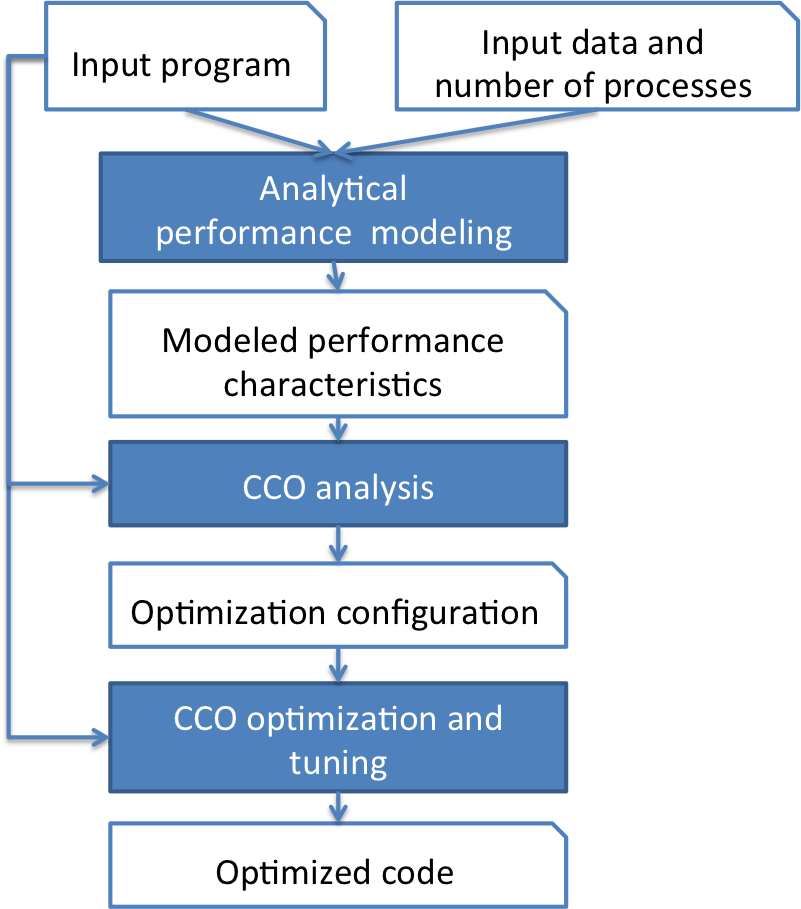
\includegraphics[width=0.35\textwidth]{fig/framework.png} % half page
\caption{Optimization workflow.}
\label{fig:overview}
\end{figure}

Figure~\ref{fig:overview} shows our workflow for systematically
enabling communication-computation overlapping (CCO) in MPI
applications to enhance their performance portability.  The
workflow contains three key components: (1) the \emph{performance
  modeling} component, which analyzes the runtime statistics of an MPI
application to extract a \emph{Bayesian execution
  tree}~\cite{jichi:ipdps14} representation of its execution flow,
including the frequencies of various runtime code paths and their
performance characteristics such as computation intensities, working
set sizes, and communication characteristics of MPI operations; (2)
the \emph{CCO analysis} component, which identifies \emph{hot}
computation and communication regions
and performs profitability and safety
analysis to determine whether to optimize these regions; and (3) the \emph{CCO
  tuning} component, which applies the appropriate program
transformations
%by replacing the blocking MPI operations with
%nonblocking ones, by reordering the computations and communications involved and by inserting
and inserts MPI\_Test operations with a frequency
determined by empirical tuning of the optimized code.
For each optimization to be profitable, any
communication slowdown from the use of the nonblocking operations must
be fully overlapped with the local computation, and the insertion of
MPI\_Test operations should cause only marginal slowdown of the computation.
% so that its effect is insignificant in comparison with the reduction of the original communication time.
Our framework currently
uses empirical tuning to select appropriate
optimization configurations and to skip nonprofitable optimizations.

The idea of overlapping computation and communication in MPI applications has been
well studied~\cite{danalis:sc05,fishgold:ipdps06}, including both using analytical performance
models~\cite{iancu:ppopp07}
and using compiler analysis~\cite{danalis:ics09} to assist the optimization.
Similar to other existing work, we also manually applied the optimizing transformations for each application.
However, our work is a step closer to complete automation than existing work in that our work fully integrates analytical performance modeling and compiler dependence analysis to automatically
determine (with optional developer guidance) the profitability and safety of the overlapping optimization. 
Furthermore, while the special interprocedural pattern of loop-based
communication-computation overlapping addressed by our work is common in scientific applications,  it has not been addressed previously in the literature.
While our example in Figure~\ref{fig:ft} contains only a singe communication inside the loop body, the optimization works similarly
when the body contains a chain of dependent communications, by overlapping them with independent computations of the previous iterations.

%Compared to using profiling to directly measure and identify code blocks to optimize,
% our analytical modeling framework is able to collectively consider all the dynamic paths through each code block,
%to more accurately identify important inter-procedural communication patterns.
Our main technical contributions are the following:

\begin{itemize}

\item Our framework tackles a common case of enhancing the overlapping of computation-communication that has not been previously addressed for MPI applications and
is able to fully automate the profitability and safety analysis of the optimization, by using advanced analytical performance
modeling (which collectively considers all the dynamic paths through each code block) and compiler dependence analysis
(which supports automated semantic inlining of developer-supplied knowledge). Developer guidance is required only to improve the
accuracy of the analysis for large scientific applications, because not all source code
of these applications is available and many low-level implementation details are impossible to fully automatically decipher~\cite{POET:ICPP11}.
 We currently manually apply the necessary program transformations,
  because code need to be carefully moved across procedural boundaries. We believe this process can be automated with some developer
guidance, which is our future work.

\item We applied our approach to optimize 7 NAS Parallel Benchmarks
  (NPB) applications on both a high-speed and a slow network-connected
  cluster environment and achieved 3--88\% speedup on both platforms.

\end{itemize}


The remainder of the paper is organized as follows.
Section~\ref{sec-model} presents our analytical performance modeling
component for automatically identifying communication and computation
hot spots in MPI applications. Section~\ref{sec-analysis} discusses how
to automatically determine the safety of the optimization through
compiler analysis.  Section~\ref{sec-opt} summarizes strategies we
used to perform the actual optimizations and the tuning of their
configurations.  Section~\ref{sec-exp} evaluates our framework using 7
NAS application benchmarks~\cite{npb}.  Section~\ref{sec-related}
discusses related work, and Section~\ref{sec-concl} presents our
conclusions.
